\begin{frame}
    \frametitle{Научная новизна}
    \begin{itemize}
    	\item Показано снижение качества работы алгоритма проекции визуальных детекций с увеличением расстояния до проецируемых препятствий.
    	\item Предложены новый алгоритмы проекции визуальных детекций на изображении на плоскость движения БTC на основе комплексирования данных с изображения и лидарного облака.
    	\item Предложены новый алгоритмы проекции сегментации  проезжей части на изображении на плоскость движения БTC на основе комплексирования данных с изображения и лидарного облака. 
        \item Предложен новый метод построения карты проходимости пространства, позволяющий снизить время задержки между моментом регистрации данных сенсором и моментом обновления карты.
    \end{itemize}
\end{frame}
\note{
    Проговаривается вслух научная новизна
}

\begin{frame}
    \frametitle{Практическая значимость}
    На результаты, полученные в работе были получены свидетельства о регистрации программ для ЭВМ и патент:
    \begin{enumerate}
    	\item №2025617212 Программное обеспечение <<Система восприятия N1 V3>>.
    	\item №2025669744 Программное обеспечение <<Способ построения карты проходимости в окрестности высокоавтоматизированного беспилотного грузового транспортного средства>>.
        \item Патент (на рассмотрении) <<Способ построения карты проходимости в окрестности высокоавтоматизированного беспилотного грузового транспортного средства>>
     \end{enumerate}
\end{frame}
\note{
    Проговариваются вслух научная и практическая значимость
}

\begin{frame}
    \frametitle{Внедрение результатов диссертационного исследования}
    \begin{figure}[h]
        \centering
        \fbox{
            \begin{minipage}[t]{0.4\linewidth}
                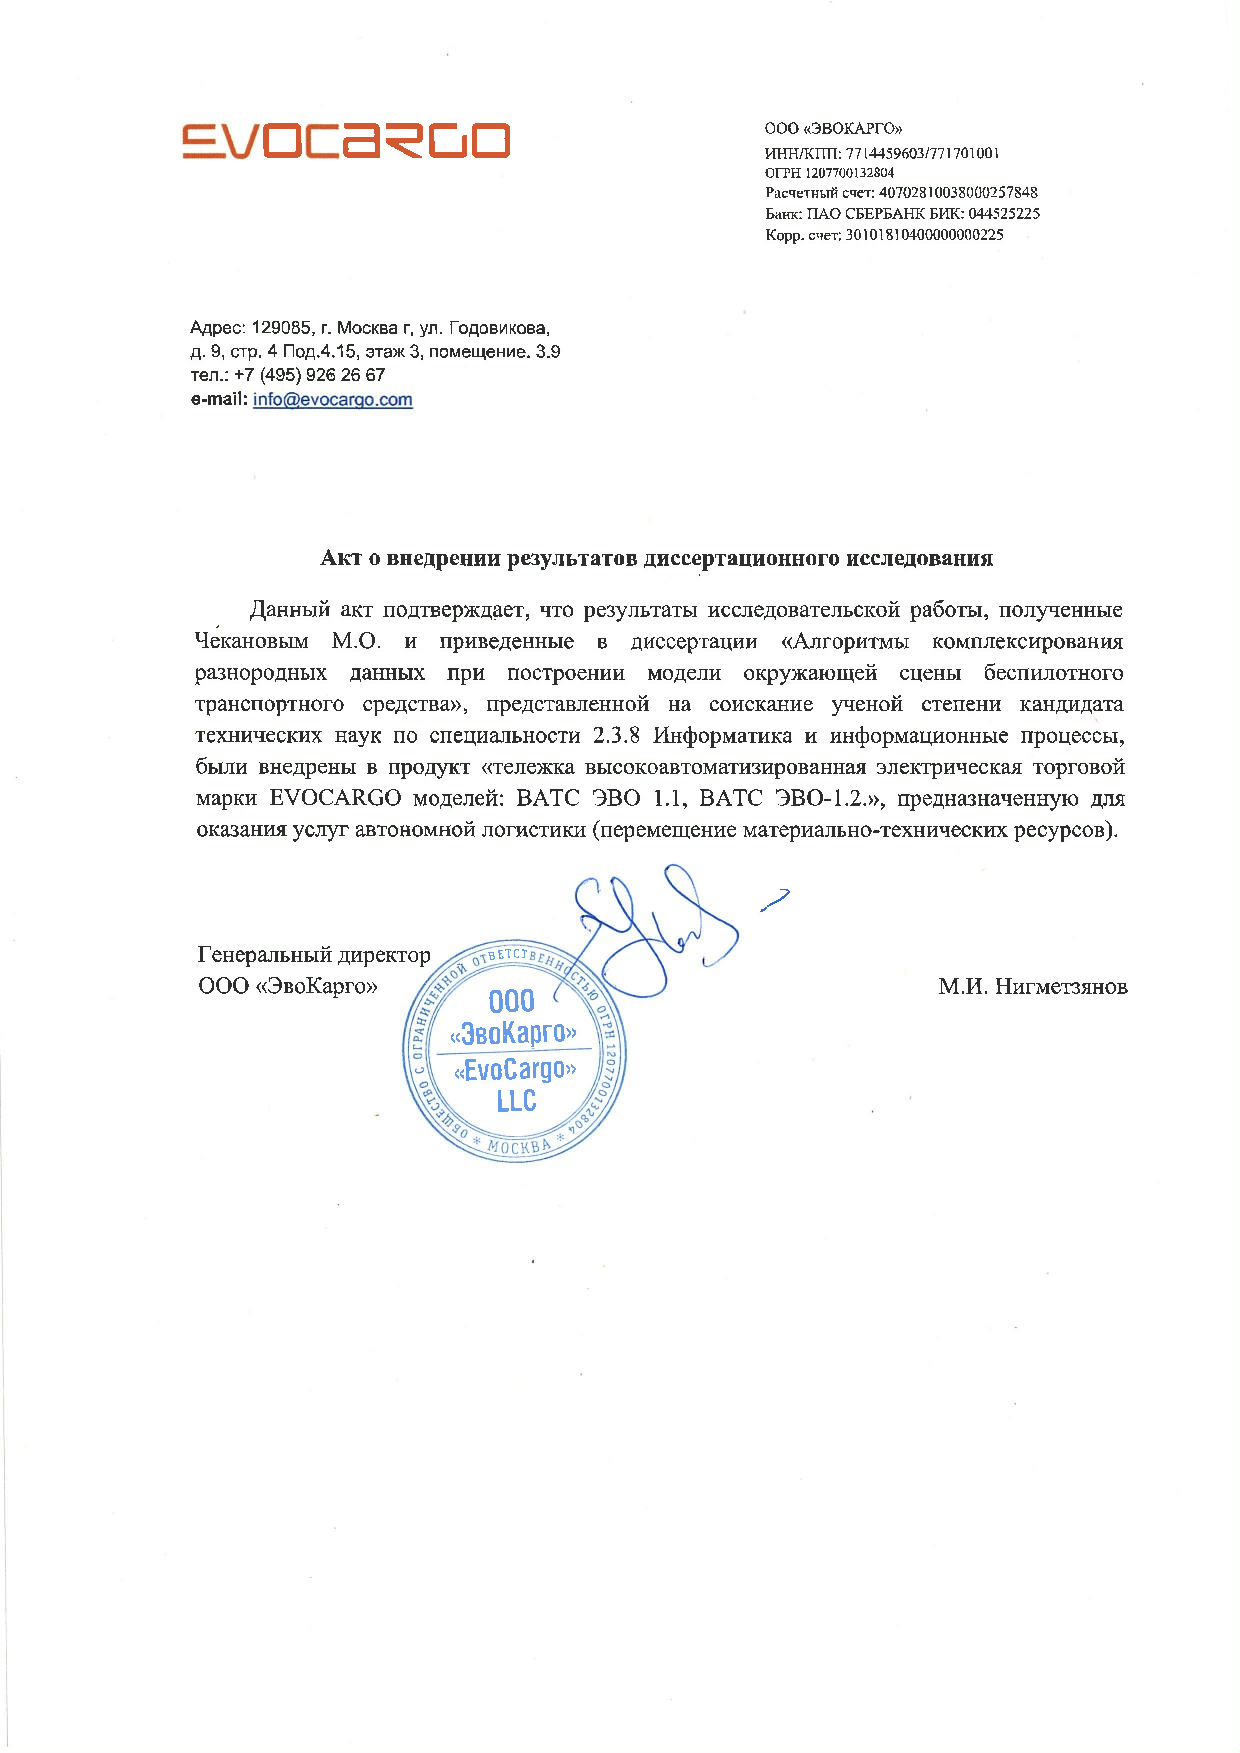
\includegraphics[width=\linewidth]{images/ChekanovAct.pdf}
            \end{minipage}
        }
    \end{figure}
\end{frame}
\note{
    Получен акт о внедрении.
}

\begin{frame} % публикации на одной странице
% \begin{frame}[t,allowframebreaks] % публикации на нескольких страницах
    \frametitle{Публикации соискателя по теме диссертационной работы}
    \begin{enumerate}
    \item \textbf{М. О. Чеканов} С. В. Кудряшова, О. С. Шипитько. Трехмерная детекция объек­тов на основе L- shape модели в автономных системах движения // \textbf{Сенсорные системы}. -- 2025. -- Т. 39, № 1. -- С. 66-78. -- DOI: 10.31857/S0235009225010078
    \item \textbf{Chekanov M. O.} L-shape fitting algorithm for 3D object detection in bird’s-eye-view in an autonomous driving system // \textbf{ICMV 2023} / Yerevan, Armenia  -- Society of Photo-Optical Instrumentation Engineers -- April 2024. -- Т. 13072. -- С. 138-145. 
    \item (на рассмотрении) \textbf{М. О. Чеканов} Многопоточные неблокирующие алгоритмы построения карты проходимости пространства // \textbf{Информационные технологии и вычислительные системы}
    \end{enumerate}
\end{frame}

\begin{frame} % публикации на одной странице
	% \begin{frame}[t,allowframebreaks] % публикации на нескольких страницах
		\frametitle{Апробация работы}
		\begin{enumerate}
			\item 16th International Conference on Machine Vision (ICMV 2023, Ереван, Армения),
		\end{enumerate}
	\end{frame}
\note{
    Работа была представлена на ряде конференций.
}

\begin{frame}[plain, noframenumbering] % последний слайд без оформления
    \begin{center}
        \Huge
        Спасибо за внимание!
    \end{center}
\end{frame}

\begin{frame}[noframenumbering]\frametitle{Модели окружающего пространства}
	В работе исследуются \textbf{двухмерные модели} – модели про­ецирующие объекты, окружающие БТС, на плоскость его движения. Как правило, этой информации достаточно для корректного планирования движения БТС.
	
	Среди существующих двумерных моделей можно выделить три категории:
	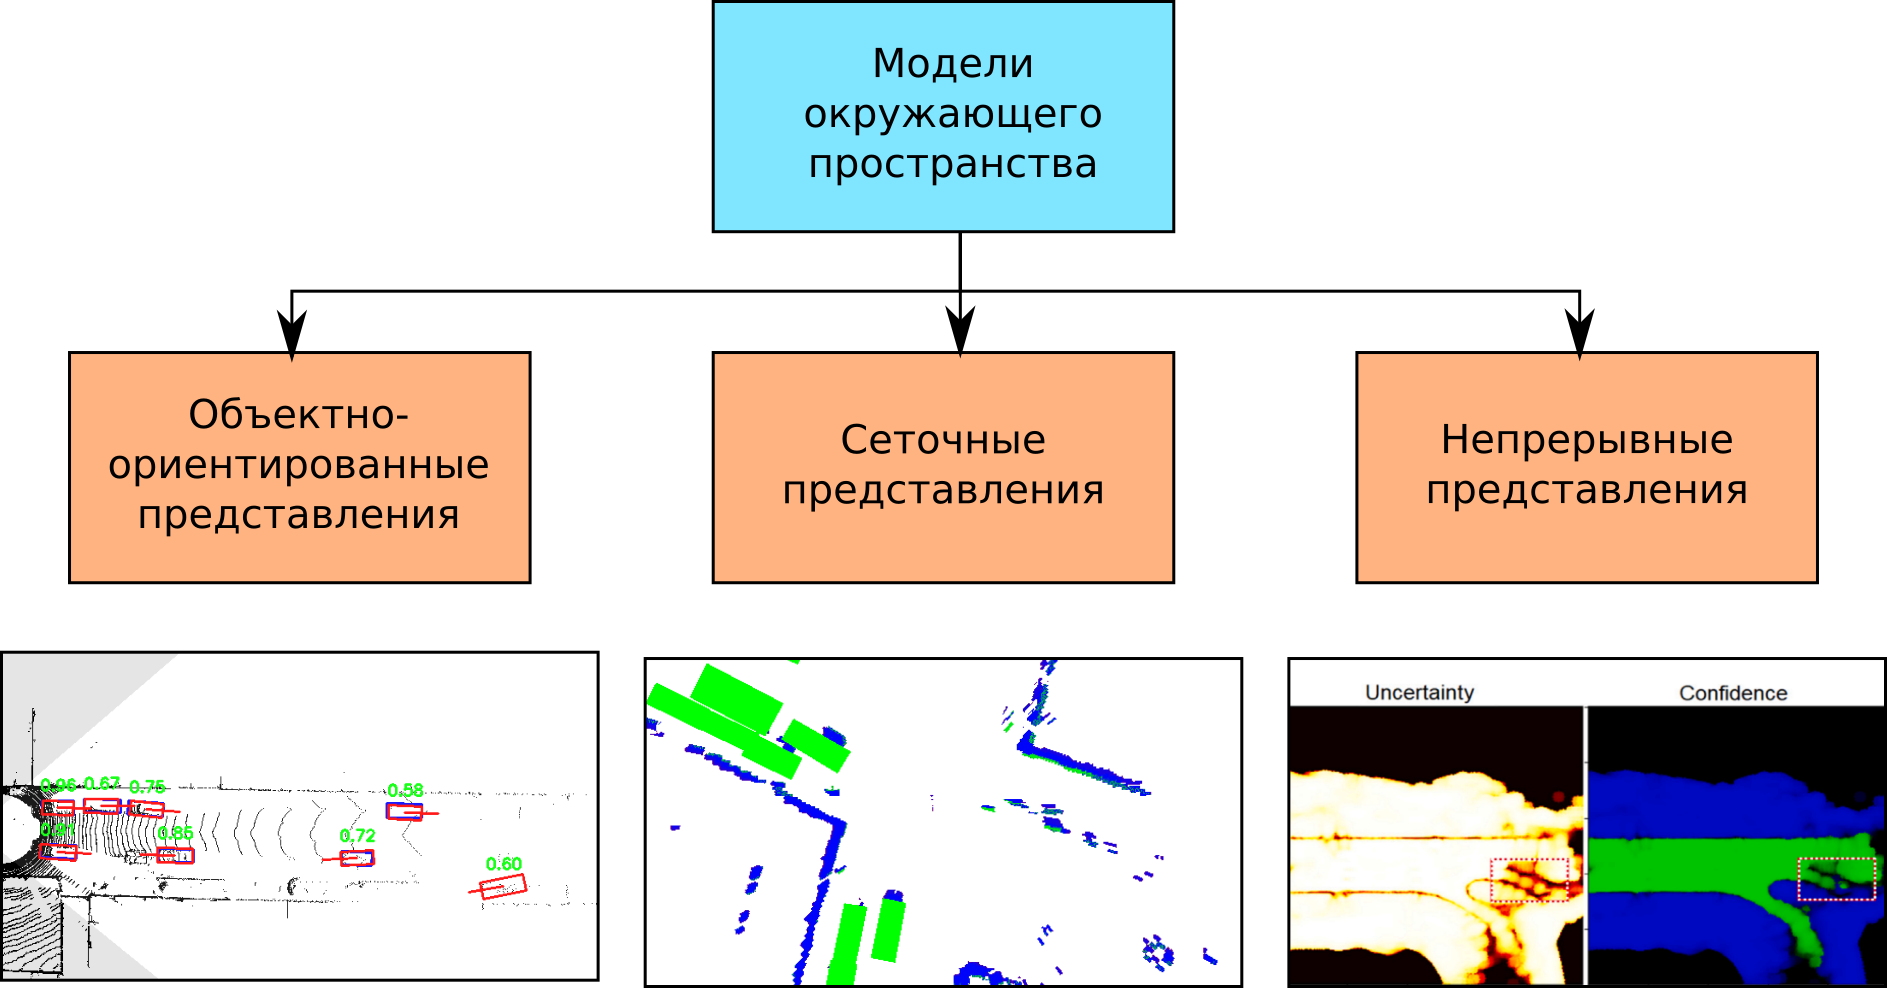
\includegraphics[width=\linewidth]{Presentation/images/models}
\end{frame}

\begin{frame}[noframenumbering]\frametitle{Алгоритм проекции сегментации проезжей части на изображении на плоскость движения БTC}
	\footnotesize
	\begin{itemize}
		\item Во втором алгоритме вычисление искомых $z(x,y)$ происходит путём добавления соответствующих точек $(x,y)$ в тестовую выборку регрессии гауссовского процесса. 
		\item \textbf{Мной был переработан} алгоритм выделения точек земли из входного облака точек, чтобы снизить время его работы.
		\item Модифицированный алгоритм позволяет выполнять одновременную регрессию на двух тестовых наборов точек с использованием механизма CUDA Streams, а также лучше использовал доступные ресурсы графического вычислителя.
		\item В результате время работы модифицированного этапа алгоритма \textbf{снизилось} с $1.5$ мс до $0.97$ мс ($-35\%$).
	\end{itemize}
	
	\begin{minipage}{0.49\linewidth}\centering
		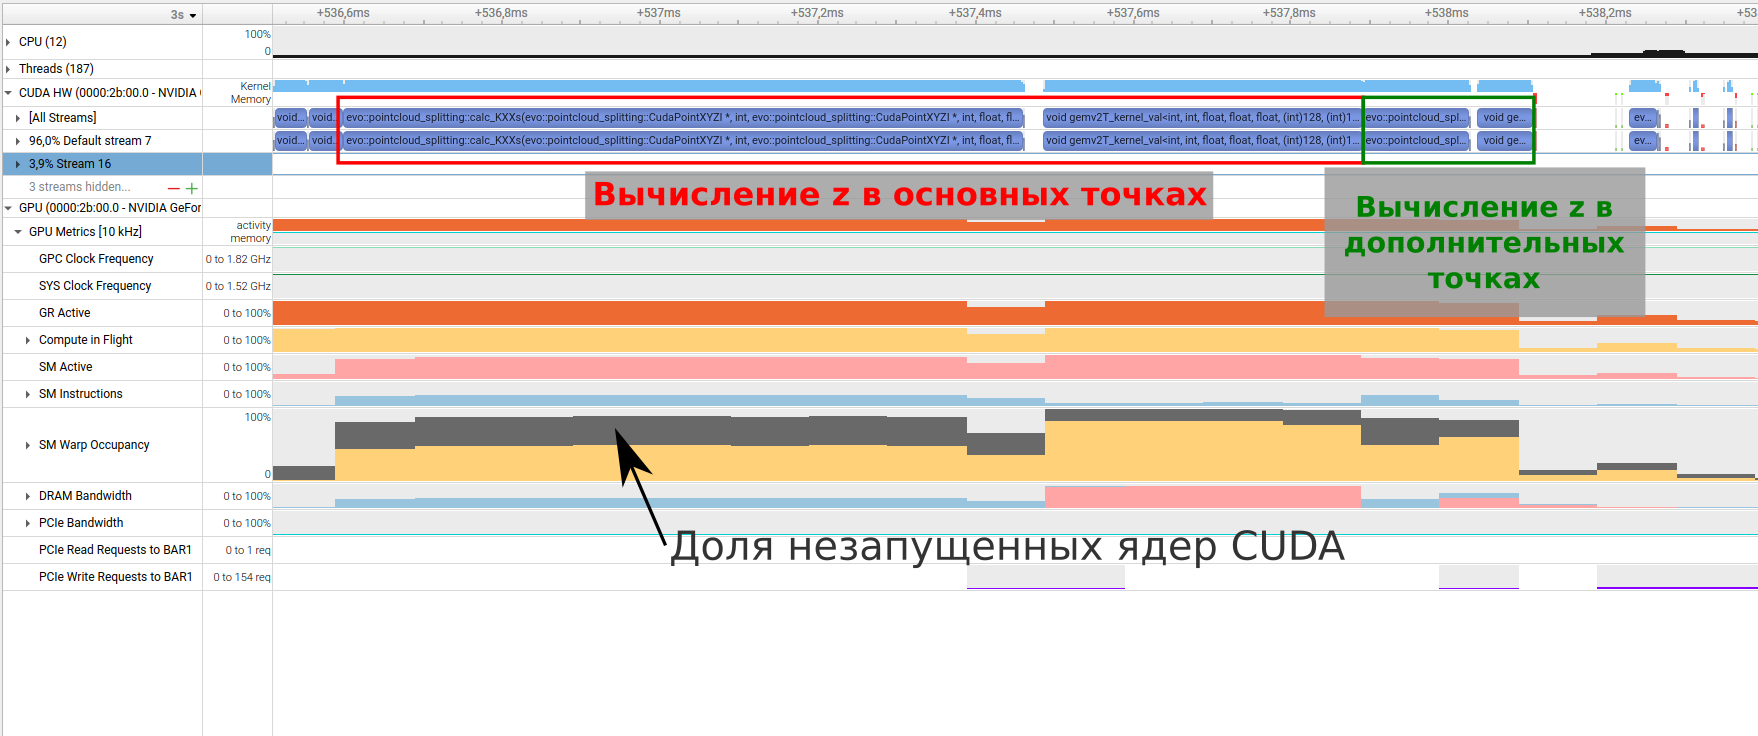
\includegraphics[width=\textwidth]{images/nsys_splitting_wo_streams} \\ а) Без использования CUDA Streams
	\end{minipage}
	\hfill
	\begin{minipage}{0.49\textwidth}\centering
		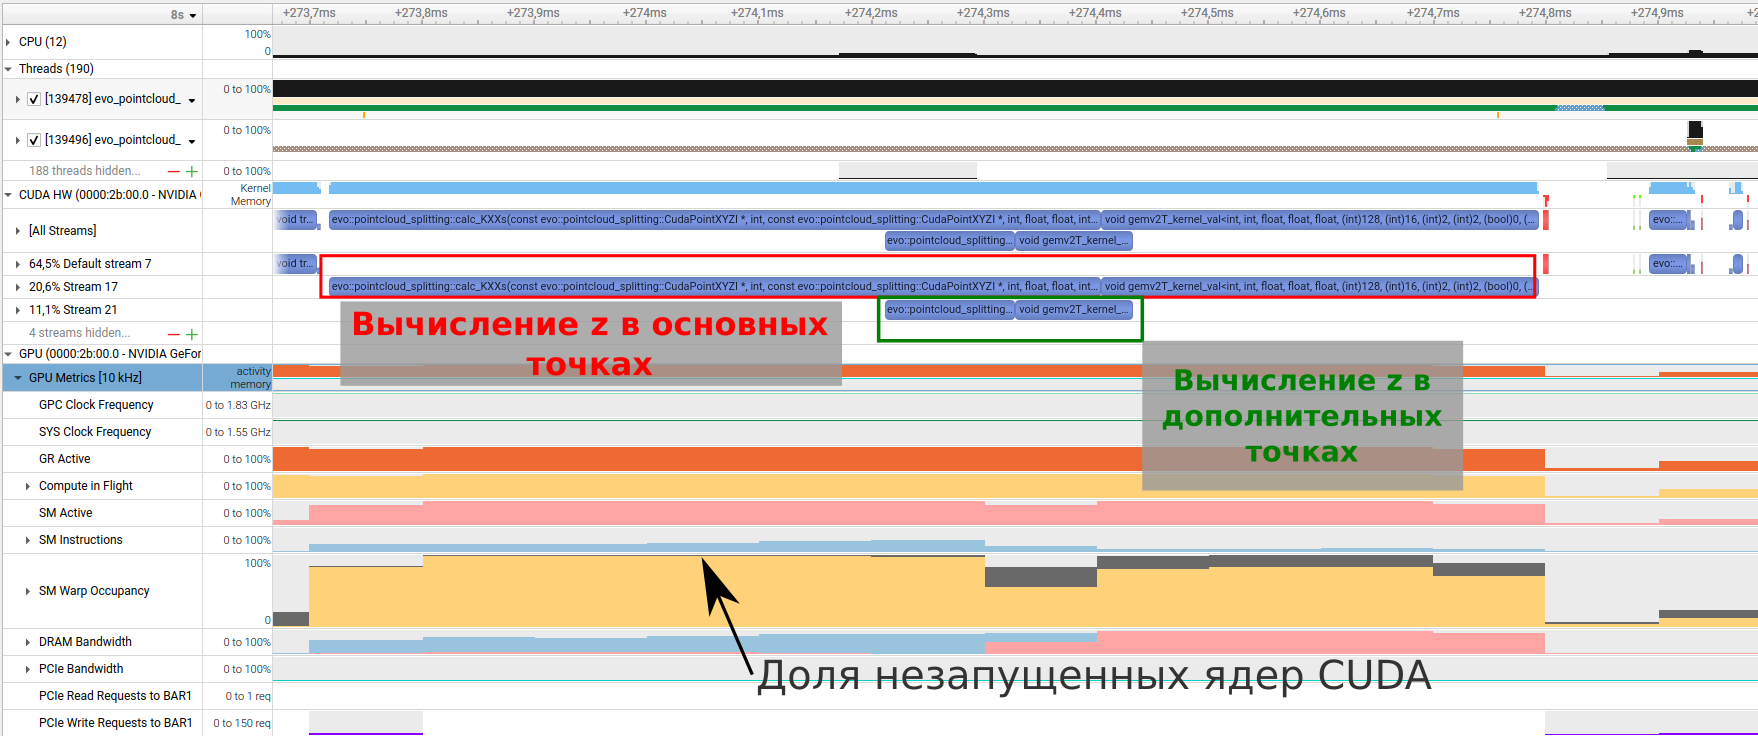
\includegraphics[width=\textwidth]{images/nsys_splitting_with_streams} \\ б) После модификации c использованием CUDA Streams
	\end{minipage}
\end{frame}
